Many web applications written today are poorly served by the databases currently
available to them. The databases are too slow to sustain the application load,
and developers are forced to implement their own ad hoc caching systems to make
the database work for them. This thesis is an attempt to improve that
situation\,---\,to build a database tailored to the particulars of these
applications that provides the performance they need.

This chapter explores the thesis motivation in greater detail
(\S\ref{s:motivation}) and briefly outlines existing solutions and their
shortcomings (\S\ref{s:existing}). It then sketches out the proposed approach
(\S\ref{s:approach}) and its implementation (\S\ref{s:intro:noria}), and
provides a list of the thesis contributions (\S\ref{s:contrib}). The chapter
concludes with a road map for how to read the remainder of the thesis
(\S\ref{s:read}).

Non-technical readers should start with Appendix~\ref{s:simple} (on
page~\pageref{s:simple}).

\section{Motivation}
\label{s:motivation}

Modern web applications typically have a number of traits in common. They are
\textbf{interactive}: each incoming request has a user waiting on the other end.
They are \textbf{read-heavy}: most interactions consume content rather than
produce new content. And they experience \textbf{significant skew}: a small
number of people, posts, teams, and discussions make up the bulk of
interactions.

Such applications are usually poorly served by the traditional relational
databases that most of them use to store and query their underlying data. These
applications tend to issue the same set of read-only queries again and again,
with the underlying data changing only infrequently. Existing databases do not
optimize for this kind of workload: they run each query in
isolation\footnote{Databases query caches~\cite{mysql-query-cache,
pgpool-query-cache} cache results as long as no changes occur to the underlying
tables if queries are byte-for-byte identical. While attractive on the surface,
they often work poorly in practice when the workload is not
read-only~\cite{mysql-query-cache-nope,pgpool-query-cache}.}, and thus re-do
work that has already been done many times over. This causes reads, which are the
most frequent operation in these applications, to be slow, while writes are
simple and fast.

\begin{figure}
  \centering
  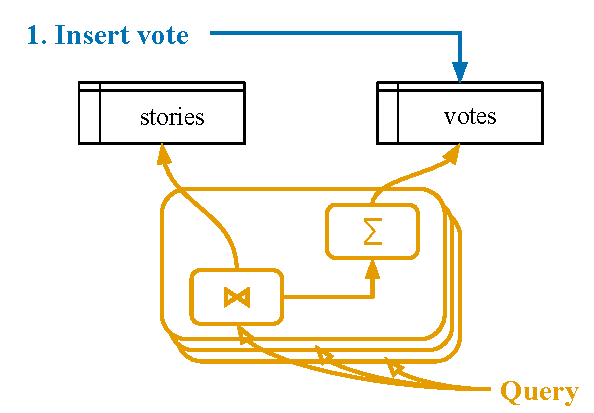
\includegraphics{diagrams/Motivation Classic DB.pdf}
  \caption{Application query execution against a traditional database. Each
  application query runs in isolation, and may perform the same work
  (\textbf{\color{set2}orange}) repeatedly. Writes do little work
  (\textbf{\color{set1}blue}), even though they are less frequent in many
  applications.}
  \label{f:motivation-classic}
\end{figure}

Figure~\vref{f:motivation-classic} shows how application queries function at a
high level in the traditional model: each query the application issues executes
the query plan, represented by an aggregation and a join in the figure. Multiple
concurrent queries execute independently, even if they run the same query.

\section{Existing Solutions}
\label{s:existing}

\begin{figure}
  \centering
  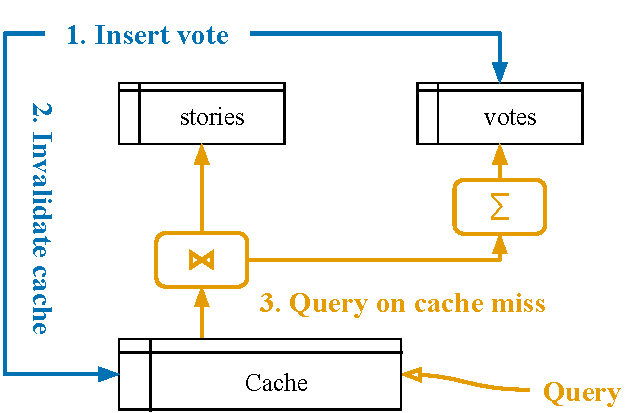
\includegraphics{diagrams/Motivation Ad Hoc Cache.pdf}
  \caption{Application query execution against a cache in front of a database.
  Application queries first check for cached results, and only execute database
  queries if the results are not cached. The application invalidates cached
  results so that later reads see the effects of new writes. The application
  logic for both reads (\textbf{\color{set2}orange}) and writes
  (\textbf{\color{set1}blue}) is more complex.}
  \label{f:motivation-adhoc}
\end{figure}

To mitigate the lackluster performance of databases for these workloads,
application authors often resort to ad hoc, error-prone
techniques~\cite{ad-hoc-caching} to exploit their applications' workload
patterns. They change their database schemas by placing and updating computed
values in the database tables, or introduce key-value stores that \textit{cache}
the result of expensive queries as shown in Figure~\vref{f:motivation-adhoc}.
All these techniques introduce significant application complexity: the
application authors must include logic to ensure that the auxiliary derived
state remains up to date as the underlying data changes, that clients do not all
flood the database when results are not available in the cache, and that
concurrent access to the database and the cache never leaves the system in an
inconsistent state.

Existing systems from industry~\cite{facebook-memcache, tao, flannel} and
academia~\cite{txcache, cachegenie, casql-consistency-thesis, pequod} have
chipped away at this problem, but are often lacking in important ways. Some
require significant developer effort, and are infeasible to implement for any
but the largest companies. Some support only a restricted set of queries, or
only provide infrastructure for developers to implement caching themselves. Many
keep the cache up to date only by evicting old results, and cannot update
existing results in-place, which is wasteful.

% Noria replaces caching \emph{logic}, not caching just caching \emph{systems}.

Eons ago~\cite{relational-materialized-views,stonebraker-views}, the database
community introduced \textit{materialized views} as an answer to the problem of
how to execute queries that are too slow to execute on demand. Materialized
views store the contents of \textit{views} (i.e., named queries) which makes
those queries faster to execute~\cite{materialized-views}. The materialized
views can then be \textit{maintained} incrementally, meaning results are updated
in-place, rather than invalidating stored results or re-executing queries from
scratch when the underlying data changes~\cite{materialized-survey}.

\begin{figure}[h]
  \centering
  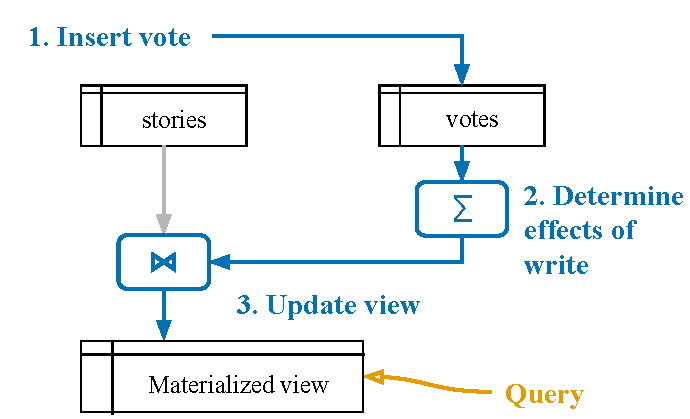
\includegraphics{diagrams/Motivation Materialized Views.pdf}
  \caption{Application query execution against a materialized view. Application
  queries only hit the view, which gives simple yet fast reads
  (\textbf{\color{set2}orange}). The database must determine the effects of
  every write and update the views to reflect changes
  (\textbf{\color{set1}blue}).}
  \label{f:motivation-materialized}
\end{figure}

Figure~\vref{f:motivation-materialized} shows an approximate architecture for an
incrementally-maintained materialized view system. The system updates the
materialized results in response to application writes, and reads access only
the stored results. Sadly, few commercially available databases support
materialized views, and the ones that do have significant
restrictions~\cite{mssql-materialized-view-restrictions}.

State-of-the-art research systems support flexible materialized
views~\cite{dbtoaster,materialize}, but do not support low-latency reads. In
these systems, reads cannot access the materialized view directly, and must
synchronize with the write-processing pipeline to get query results. Many of
these systems are also restricted to a predeclared set of queries, and cannot
incorporate changes to application queries without restarting.

Most materialized view systems do not have the ability to evict infrequently
accessed state that accumulates over time. They thus function poorly as a
replacement for a cache: infrequently accessed results cannot be evicted, and
reads must wait on writes. Dynamic materialized
views~\cite{dynamic-materialized-views, partially-materialized-views} allow the
application to materialize only a subset of each view. This enables limited
eviction, but is cumbersome for the application to manage, and only allows
coarse-grained eviction decisions (\S\ref{s:disc:emulating}).

\section{Approach: Partial State}
\label{s:approach}

Materialized views represent an ``almost there'' solution to automatic caching.
They provide a great foundational mechanism for storing and maintaining query
results efficiently in a way that meshes well with how applications already
work: by issuing SQL queries. What is missing to make materialized views a
viable replacement for the ad hoc caching strategies today's applications employ
is a way to make the materialized views more dynamic. Specifically, to serve as
a good cache-substitute, materialized views must support efficiently adding new
queries and evicting old results at runtime.

To bridge the gap, this thesis proposes \textit{partially materialized
state}\footnote{The database literature sometimes refers to a view where only
some columns are materialized as ``partially
materialized''~\cite{partially-materialized}. This meaning of the term is
unrelated to the use of the term in this thesis.}, or partial state for short.
Partial state lets entries in materialized views be marked as \textit{missing},
and introduces \textit{upqueries} to compute such missing state on-demand.
This allows new queries to be added efficiently by leaving the initial
materialized view empty, and populating the view only in response to application
queries. Furthermore, as the application loses interest in old query results,
those results can be evicted to reclaim memory, which can in turn be used to
cache more important query results. In essence, partial state enables
materialized views to function like caches.

In the proposed work, the system model still looks like
Figure~\vref{f:motivation-materialized}, except that the materialized view also
contains parameters whose value the application supplies at runtime. Queries to
the materialized view can then \emph{miss} for a given parameter value, just
like in a cache. When they do, the database internally fills in the missing
state before it responds to the application. If the application later executes
the same query, the cache holds the result. Over time, the database evicts
infrequently accessed results to save memory and to avoid the overhead of
maintaining results the application is no longer interested in.

\section{Partial State in Noria}
\label{s:intro:noria}

The thesis includes an implementation of partial state in Noria, a
state-of-the-art materialized view system that is already optimized for
read-heavy, dynamic web applications~\cite{noria}. Noria uses \textit{dataflow}
internally to maintain its materialized views, a system architecture that allows
fast and distributed computation over a stream of data changes. Dataflow
represents computational dependencies as a directed acyclic graph where edges
represent data dependencies, and vertices represent computations (like
aggregations or joins) over the data that arrives over the incoming edges.
Partial state upqueries flow ``up'' this dataflow, in the opposite direction of
the data, and trigger the retransmission of past state in the case of a cache
miss. The resulting retransmissions then use the existing Noria dataflow to
process the responses and fill in missing state. This avoids the need for
separate logic for serving cache misses and maintaining already cached state,
and simplifies the implementation.

\section{Contributions}
\label{s:contrib}

The main contributions of this thesis are:

\begin{itemize}
 \item A model for, and implementation of, partial state in a dataflow-based
   materialized view system.
 \item Upqueries\,---\,a mechanism that populates missing state on demand.
 \item An analysis of the inconsistencies that arise when introducing partial
   state to a distributed, high-performance stateful dataflow processing system
    where updates can race with one another, and with upqueries.
 \item Techniques for overcoming those inconsistencies while preserving system
   correctness, performance, and scalability.
 \item Micro and macro evaluations of the performance and memory benefits of
   partial state. Experimental results suggest that the presented system
    increases supported application load by up to $20\times$ over MySQL, and
    reduces memory use by up to $\sfrac{2}{3}$ compared to existing approaches.
\end{itemize}

\paragraph{Limitations.}
The presented system is not without limitations: it is eventually consistent
(\S\ref{s:noria:consistency}), supports only a subset of SQL
(\S\ref{s:noria:sql}), increases memory use (\S\ref{s:eval:why}), and reduces
write performance (\S\ref{s:eval:writes}). Chapters~\ref{s:disc} and
\ref{s:future} discuss possible avenues for mitigating some of these
shortcomings.

\section{Reading Guide}
\label{s:read}

The rest of the dissertation is organized as follows: Chapter~\ref{s:noria}
describes the Noria dataflow system. Chapter~\ref{s:partial} introduces the
partially stateful dataflow model. Chapter~\ref{s:correct} describes additional
mechanisms that are needed to ensure that partially stateful dataflow produces
correct query results. Chapter~\ref{s:impl} details some of the implementation
decisions in the thesis prototype. Chapter~\ref{s:eval} evaluates Noria's
implementation of partial state on a realistic application query workload.
Chapter~\ref{s:related} explores related work. Chapter~\ref{s:disc} discusses
shortcomings of, and alternatives to, partial state. Finally,
Chapter~\ref{s:future} outlines future work on partial state.

For readers that are unfamiliar with database queries, materialized views,
dataflow, and application caching, but would still like to understand roughly
what this thesis is about, Appendix~\ref{s:simple} starting on
page~\pageref{s:simple} is for you.
